\documentclass{beamer}
\usetheme{Madrid}

% pdflatex
\usepackage[utf8]{inputenc}
\usepackage[T2A]{fontenc}
\usepackage[russian,english]{babel}
\usepackage{cmap}
% \usepackage{lmodern}

\usepackage{graphicx}
\usepackage{xcolor}
\usepackage{tikz}
\usepackage{amsmath,amssymb,amsthm}
\usepackage{mathtools}
\usepackage{listings}
\usepackage{booktabs}
\usepackage{array}
\usetikzlibrary{arrows.meta,positioning,shapes.geometric,fit,backgrounds,calc,decorations.pathreplacing}

% ...existing code...

% Footline: show current section (left) and frame numbers (right)
\setbeamertemplate{footline}{%
  \leavevmode%
  \hbox{%
    \begin{beamercolorbox}[wd=.78\paperwidth,ht=2.5ex,dp=1ex,left]{author in head/foot}%
      \hspace*{1em}\usebeamerfont{footline}\insertsectionhead%
    \end{beamercolorbox}%
    \begin{beamercolorbox}[wd=.22\paperwidth,ht=2.5ex,dp=1ex,right]{date in head/foot}%
      \usebeamerfont{footline}\insertframenumber{} / \inserttotalframenumber\hspace*{1em}%
    \end{beamercolorbox}%
  }%
}

\newcommand{\parpause}[1]{\only<+->{#1\par}}
\newenvironment{definitionbox}[1][Определение]{%
  \begin{exampleblock}{#1}
}{%
  \end{exampleblock}
}

% Math shortcuts
\newcommand{\sqcupLUB}{\sqcup}
\newcommand{\leqpo}{\leq}
\newcommand{\merge}{\mathbin{\sqcup}}
\newcommand{\ts}{\mathit{ts}}

\AtBeginSection[]
{
  \begin{frame}
    \frametitle{Содержание}
    \tableofcontents[currentsection]
  \end{frame}
}

\title{Семинар 8. CRDT для последовательностей и CALM-теорема}
\subtitle{Распределенные вычисления}
\author{Георгий Семенов}
\institute{Институт прикладных компьютерных наук \\ Университет ИТМО}
\date{весна 2026}

\begin{document}

\frame{\titlepage}

\begin{frame}
\frametitle{Организационные моменты}

\begin{itemize}
  \item Третье домашнее задание – автопроверка \\ (10 баллов = 2 + 2 + 4 + 2)
  \item Проставлю баллы по зеленым галочкам в GitHub Classroom
\end{itemize}

\end{frame}

%--------------------------------------------------
\section{Другие структуры данных}

\begin{frame}
\frametitle{Add-only Monotonic DAG}

\textbf{CRDT-граф:} добавление вершин и рёбер, без удаления. Реализуется как два G-Set: $V$ (вершины), $E$ (рёбра).

\medskip
\textbf{Свойство монотонности DAG:} при добавлении ребра $(u,v)$ — предикат проверяется \emph{локально}; merge может нарушить DAG-условие (отсутствие циклов), поэтому часто используют \textbf{только partial order} как инвариант.

\begin{center}
\begin{tikzpicture}[scale=0.85, every node/.style={font=\scriptsize},
  node/.style={draw,circle,fill=blue!20,minimum size=0.55cm}]
  \node[node] (a) at (0,1.5) {a};
  \node[node] (b) at (1.5,1.5) {b};
  \node[node] (c) at (3,1.5) {c};
  \node[node] (d) at (1.5,0) {d};
  \draw[->,thick](a)--(b); \draw[->,thick](b)--(c);
  \draw[->,thick](a)--(d); \draw[->,thick](d)--(c);

  \node[font=\tiny,align=left] at (5.5,0.9)
    {Replica 1:\\add edge $(b,d)$};
  \node[font=\tiny,align=left] at (5.5,0.3)
    {Replica 2:\\add vertex $e$, add edge $(c,e)$};

  \node[node,fill=orange!20] (e) at (4.5,1.5) {e};
  \draw[->,thick,dashed,orange](c)--(e);
  \draw[->,thick,dashed,blue](b) to[bend right=20] (d);
\end{tikzpicture}
\end{center}

\textbf{Применение:} системы контроля версий (commit graph), workflow engines, causality tracking.

\end{frame}

\begin{frame}
\frametitle{Causal Tree и 2P-Set Graph}

\begin{columns}
\begin{column}{0.48\textwidth}
\begin{block}{Causal Tree (CT)}
\begin{itemize}
  \item Каждая операция — узел дерева с ссылкой на \textbf{причину} (parent op)
  \item Структура: $\{(id, \text{parent\_id}, \text{payload})\}$
  \item Базис для WOOT, RGA, Treedoc
  \item Tombstone: удалённые узлы маркируются, но не удаляются
  \item Исп. в Atom Teletype, xi-editor
\end{itemize}
\end{block}
\end{column}
\begin{column}{0.48\textwidth}
\begin{block}{2P-Set Graph}
\begin{itemize}
  \item Два 2P-Set: $V$ (вершины), $E$ (рёбра)
  \item \texttt{addVertex}, \texttt{addEdge}, \texttt{removeVertex}, \texttt{removeEdge}
  \item Инвариант: $e=(u,v) \in E \Rightarrow u \in V \land v \in V$
  \item Поддержание инварианта при merge — сложность
  \item Shapiro et al. (2011) предлагают \textbf{vertex-removal precondition}
\end{itemize}
\end{block}
\end{column}
\end{columns}

\end{frame}

\section{Немного про последовательности}

\begin{frame}
\frametitle{WOOT (Without Operational Transformation)}

\begin{columns}
\begin{column}{0.52\textwidth}
\textbf{Каждый символ:} $\langle id, v, W_L, W_R, \text{visible}\rangle$
\begin{itemize}
  \item $id$ — уникальный идентификатор (сайт, clock)
  \item $W_L$, $W_R$ — соседи \emph{в момент вставки}
  \item При merge: вставляем символ, используя $W_L$, $W_R$ для определения позиции
  \item Конкурентные вставки в одну позицию разрешаются детерминированным tiebreaking по $id$
\end{itemize}
\end{column}
\begin{column}{0.45\textwidth}
\begin{tikzpicture}[scale=0.80, every node/.style={font=\scriptsize}]
  % Document sequence
  \node[font=\small] at (1.5, 3.2) {Документ: \texttt{[B·E·G·I·N]}};
  \foreach \c/\x in {B/0, E/0.7, G/1.4, I/2.1, N/2.8}{
    \node[draw,minimum size=0.5cm,fill=blue!15] at (\x,2.5) {\c};
  }
  % Insert H between G and I
  \draw[->,red,thick] (1.4,2.0) -- (1.75,2.25);
  \node[draw,minimum size=0.5cm,fill=red!25] at (1.75,1.5) {H};
  \node[font=\tiny,red,align=center] at (3.0,1.0) {insert H\\between G,I};
  \node[font=\tiny,align=center] at (1.5,0.3)
    {Result: B·E·G·H·I·N};
\end{tikzpicture}
\end{column}
\end{columns}

\textbf{Сложность:} $O(n^2)$ на вставку в худшем случае (много конкурентных вставок).

\end{frame}

\begin{frame}
\frametitle{RGA (Replicated Growable Array)}

\textbf{Идея:} связный список с уникальными s4vector $(s, sum, sid, seq)$

\begin{columns}
\begin{column}{0.52\textwidth}

\begin{itemize}
  \item Каждый элемент: $\langle s4, v, \text{next}, \text{deleted}\rangle$
  \item Вставка: находим predecessor по s4, вставляем после него
  \item При конфликте (два insert после одного и того же): сортировка по s4 (timestamp desc)
  \item Tombstone для удалений (элемент остаётся в списке, маркируется)
\end{itemize}

\end{column}
\begin{column}{0.45\textwidth}

\begin{center}
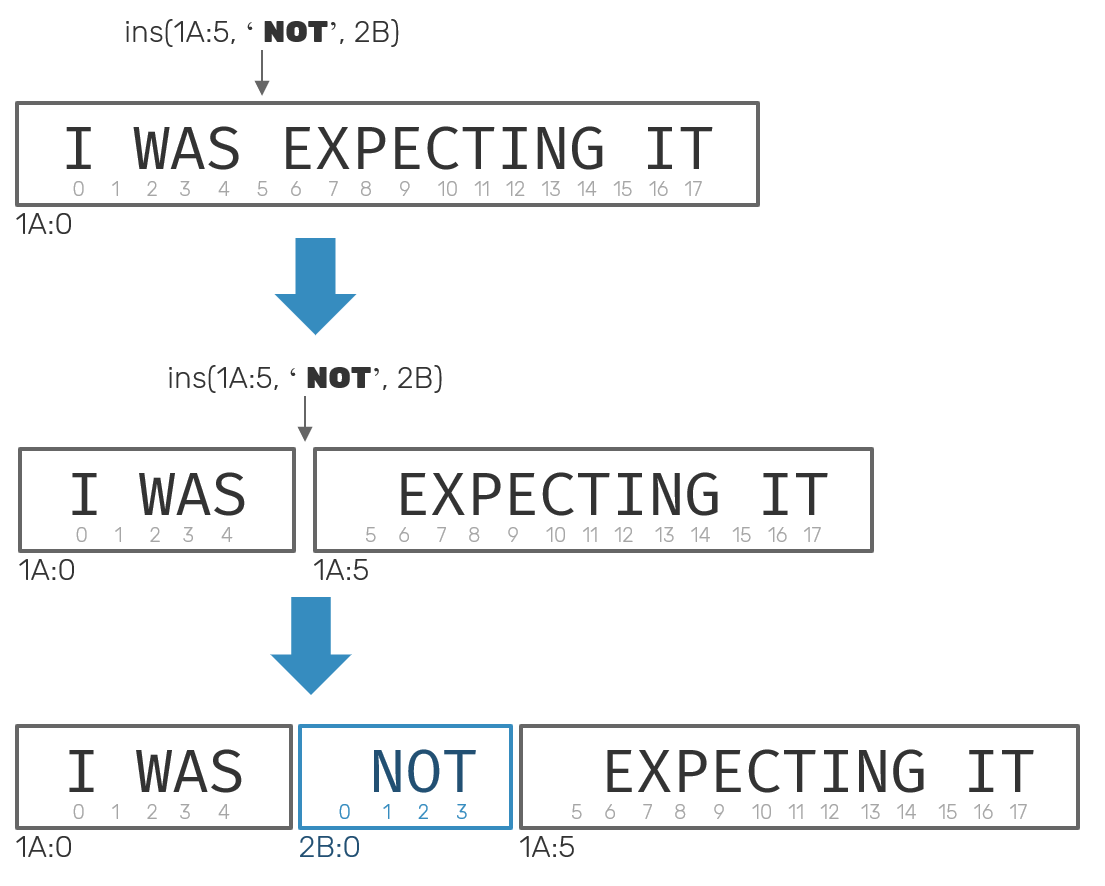
\includegraphics[width=1.0\linewidth,keepaspectratio]{./images/blockwise-rga-insert.png}
\end{center}

\end{column}
\end{columns}

\medskip
\textbf{Применения:} Riak DT, Automerge (ранняя версия), Yjs (частично).
\textbf{Сложность:} $O(n)$ для вставки, $O(1)$ амортизированного для конвергентных вставок.

\end{frame}

\begin{frame}
\frametitle{Logoot и LSEQ}

\begin{columns}
\begin{column}{0.52\textwidth}
\textbf{Logoot:} каждому элементу присваивается \textbf{уникальный позиционный идентификатор} из упорядоченного пространства $\mathcal{I}$.
\begin{itemize}
  \item $id = [(p_1, s_1), (p_2, s_2), \ldots]$ — список пар (позиция, сайт)
  \item Вставка между $id_L$ и $id_R$: выбрать $id$ с $id_L < id < id_R$
  \item Документ = упорядоченное множество $(id, v)$ пар
  \item Удаление: просто удалить по $id$
\end{itemize}

\medskip
\textbf{LSEQ:} адаптивное выделение идентификаторов для контроля длины пути — решает проблему «надувания» id в Logoot.
\end{column}
\begin{column}{0.45\textwidth}
\begin{tikzpicture}[scale=0.75, every node/.style={font=\scriptsize}]
  \node at (1.5,3.8) {\textbf{Идентификаторный интервал}};
  \draw[thick,->] (0,3) -- (3.2,3) node[right] {$\mathcal{I}$};
  \node[below] at (0,3) {$-\infty$};
  \node[below] at (3,3) {$+\infty$};

  \node[draw,circle,fill=blue!25,inner sep=1pt] (a) at (0.8,3) {};
  \node[draw,circle,fill=blue!25,inner sep=1pt] (b) at (2.4,3) {};
  \node[below,font=\tiny] at (0.8,2.9) {$id_L$};
  \node[below,font=\tiny] at (2.4,2.9) {$id_R$};

  \node[draw,circle,fill=red!40,inner sep=1pt] (c) at (1.6,3) {};
  \node[above,font=\tiny,red] at (1.6,3.05) {new $id$};

  \draw[<->,thick,blue] (0.8,2.0) -- (2.4,2.0) node[midway,below,font=\tiny]{free space};

  \node[font=\tiny,align=center] at (1.5,0.0)
    {LSEQ: адаптивно\\ чередует стратегии\\boundary+ / boundary-\\для balance дерева};
\end{tikzpicture}
\end{column}
\end{columns}

\end{frame}

\begin{frame}
\frametitle{Treedoc}

\begin{columns}
\begin{column}{0.52\textwidth}
\textbf{Идея:} последовательность как бинарное дерево с \emph{in-order traversal}.

\begin{itemize}
  \item Узел дерева = элемент + уникальный $id$ (путь в дереве)
  \item Идентификатор пути естественно упорядочен: in-order traversal
  \item Вставка между $L$ и $R$: добавить узел как левый потомок следующего или правый потомок текущего
  \item \textbf{Disambiguator} (site id) для конкурентных вставок в один узел (mini-tree)
\end{itemize}
\end{column}
\begin{column}{0.45\textwidth}
\begin{tikzpicture}[scale=0.78, every node/.style={font=\scriptsize},
  nd/.style={draw,circle,fill=blue!20,minimum size=0.55cm}]
  \node[nd] (r) at (2,3.5) {m};
  \node[nd] (l) at (0.8,2.4) {a};
  \node[nd] (rr) at (3.2,2.4) {z};
  \node[nd] (lr) at (1.6,1.3) {n};
  \draw[-,thick](r)--(l); \draw[-,thick](r)--(rr);
  \draw[-,thick](l)--(lr);

  \node[font=\tiny,align=center] at (2,0.5)
    {in-order: a, m, n, z\\(document order)};
  \node[nd,fill=red!20] (ins) at (2.5,1.3) {o};
  \draw[-,thick,dashed,red](rr)--(ins);
  \node[font=\tiny,red,align=center] at (4.5,1.5) {insert 'o'\\after 'n'};
\end{tikzpicture}
\end{column}
\end{columns}

\medskip
\textbf{Компакция:} tombstone-узлы без потомков удаляются при synchronization — уникальность CRDT!


\end{frame}

\begin{frame}
\frametitle{Chronofold}

\begin{columns}
\begin{column}{0.55\textwidth}
\textbf{Ключевые идеи:}
\begin{itemize}
  \item Хранить операции в \textbf{chrono-order} (timestamp), не в document order
  \item \textbf{Implicit linked list:} поддерживается массив «следующих» указателей $\mathit{nxt}[\cdot]$
  \item Document order восстанавливается обходом implicit list за $O(n)$
  \item Вставка новой операции: $O(1)$ амортизированно при FIFO доставке
\end{itemize}

\medskip
% \textbf{Формально:}\\
% $\text{CF} = (A, \mathit{nxt}, \mathit{ref})$ где:
% \begin{itemize}
%   \item $A[t]$ — операция с таймером $t$
%   \item $\mathit{ref}[t]$ — $t$ ссылается на предыдущую операцию
%   \item $\mathit{nxt}[t]$ — implicitly maintained sibling list
% \end{itemize}

\end{column}
\begin{column}{0.42\textwidth}
\begin{tikzpicture}[scale=0.78, every node/.style={font=\scriptsize}]
  \node[font=\small] at (1.5,4.5) {\textbf{Chrono order} (массив)};
  \foreach \t/\c/\x in {1/H/0, 2/e/0.8, 3/l/1.6, 4/p/2.4, 5/!/3.2}{
    \node[draw,fill=blue!15,minimum size=0.55cm] at (\x,2.8) {\c};
    \node[font=\tiny] at (\x, 3.6) {$t=\t$};
  }
  % nxt pointers (document order via linked list)
  % Suppose insert 'l2' at t=6 after t=2 (ref=e)
  \node[draw,fill=red!20,minimum size=0.55cm] at (0,2.0) {l};
  \node[font=\tiny,red] at (0,1.55) {$t=6$, ref=2};
  \draw[->,red,thick,bend right=20] (0,1.8) to node[left,font=\tiny]{nxt} (0.8,3.0);
  \node[font=\tiny,align=center] at (1.8,1.0)
    {Document order:\\H·e·l·l·p·!\\(follow nxt links)};
\end{tikzpicture}
\end{column}
\end{columns}

\end{frame}

\begin{frame}
\frametitle{Fugue и FugueMax}

\begin{columns}
\begin{column}{0.55\textwidth}
\textbf{Мотивация:}\\
Существующие CRDT для последовательностей (RGA, YATA, Logoot) не имеют \textbf{формальных гарантий качества порядка} при конкурентных вставках. Вводится понятие \textbf{non-interleaving}.

\medskip
\begin{definitionbox}[Non-interleaving]
\small Пусть пользователи A и B конкурентно вставляют последовательности символов $a_1\ldots a_k$ и $b_1\ldots b_m$ в одну позицию. CRDT \emph{не перемежает} их, если итоговый порядок — либо $a_1\ldots a_k b_1\ldots b_m$, либо $b_1\ldots b_m a_1\ldots a_k$.
\end{definitionbox}

\end{column}
\begin{column}{0.42\textwidth}
\textbf{FugueMax:}\\
Расширение с явным понятием «maximal non-interleaving» — оптимально для UX.

\medskip
\begin{tikzpicture}[scale=0.80, every node/.style={font=\scriptsize}]
  \node[draw,fill=blue!15,rounded corners,align=center] at (0.7,2.3)
    {A вставляет\\``foo''};
  \node[draw,fill=red!15,rounded corners,align=center] at (3.5,2.3)
    {B вставляет\\``bar''};
  \node[draw,fill=green!20,rounded corners,align=center] at (2.0,0.75)
    {Fugue:\\``foobar'' или ``barfoo''\\(не ``fbaoor'')};

  \node[draw,fill=orange!20,rounded corners,align=center] at (2.0,-1.0)
    {RGA может дать:\\``fboaor'' ← плохо!};
\end{tikzpicture}
\end{column}
\end{columns}

\medskip
\textbf{Результат:} RGA, Logoot, LSEQ — \emph{нарушают} non-interleaving. Fugue — \textbf{гарантирует}.


\end{frame}

\section{CALM-теорема}

\begin{frame}
\frametitle{CALM-теорема: Consistency As Logical Monotonicity}

\begin{columns}
\begin{column}{0.6\textwidth}
\textbf{Основная идея (Hellerstein et al., 2010):}

Программа достигает консистентности без координации $\Leftrightarrow$ её логика \emph{монотонна}.



\end{column}
\begin{column}{0.3\textwidth}
\begin{tikzpicture}[scale=0.85, every node/.style={font=\scriptsize}]
  \node[draw,fill=blue!15,rounded corners,align=center,minimum width=3.5cm] at (0,2.2)
    {Monotonic logic\\(order-insensitive)};
  \node[draw,fill=green!20,rounded corners,align=center,minimum width=3.5cm] at (0,1.0)
    {Convergent\\without coordination};
  
  \node[draw,fill=red!15,rounded corners,align=center,minimum width=3.5cm] at (0,-1.0)
    {Non-monotonic logic\\(order-sensitive)};
  \node[draw,fill=orange!20,rounded corners,align=center,minimum width=3.5cm] at (0,-2.2)
    {Needs coordination};
\end{tikzpicture}
\end{column}
\end{columns}

\end{frame}


\section{Итоги}

\begin{frame}
\frametitle{Открытые проблемы}

\begin{exampleblock}{Открытые вопросы}
\small
\begin{itemize}
  \item Delta-CRDT (меньше трафика, Almeida et al., 2018)
  \item Pure op-based CRDT (Baquero et al., 2017)
  \item CRDT в БД: Electric SQL, Ditto, Automerge 2.0
\end{itemize}
\end{exampleblock}

\end{frame}

\begin{frame}
\frametitle{Итоги}

\begin{itemize}
\item Выдано 3-е домашнее задание про CRDT.
\end{itemize}


\end{frame}

\end{document}